\section{Metodología de investigación aplicada}
\subsection{Diseño}
Se empleó un diseño de investigación-acción con ciclos planificar–actuar–observar–reflexionar, complementado con estudio de caso sobre el desarrollo y la puesta en marcha de UrbanTracker. Se fijaron principios (simplicidad, bajo costo, escalabilidad), criterios de éxito (actualización en ~5 s y latencia <2 s del móvil a la web, panel usable) y un plan de evaluación que combinó verificaciones funcionales y mediciones extremo a extremo.

\subsection{Comparación de metodologías ágiles}
Para seleccionar prácticas ágiles se realizó una evaluación multi-criterio (claridad de roles, cadencia, facilidad de adopción, riesgo). El resultado inclinó la balanza hacia Scrum (iteraciones cortas, roles definidos) con prácticas de Kanban (flujo visual y límites de WIP) para el trabajo operativo continuo.

\begin{figure}[htbp]
    \centering
    % 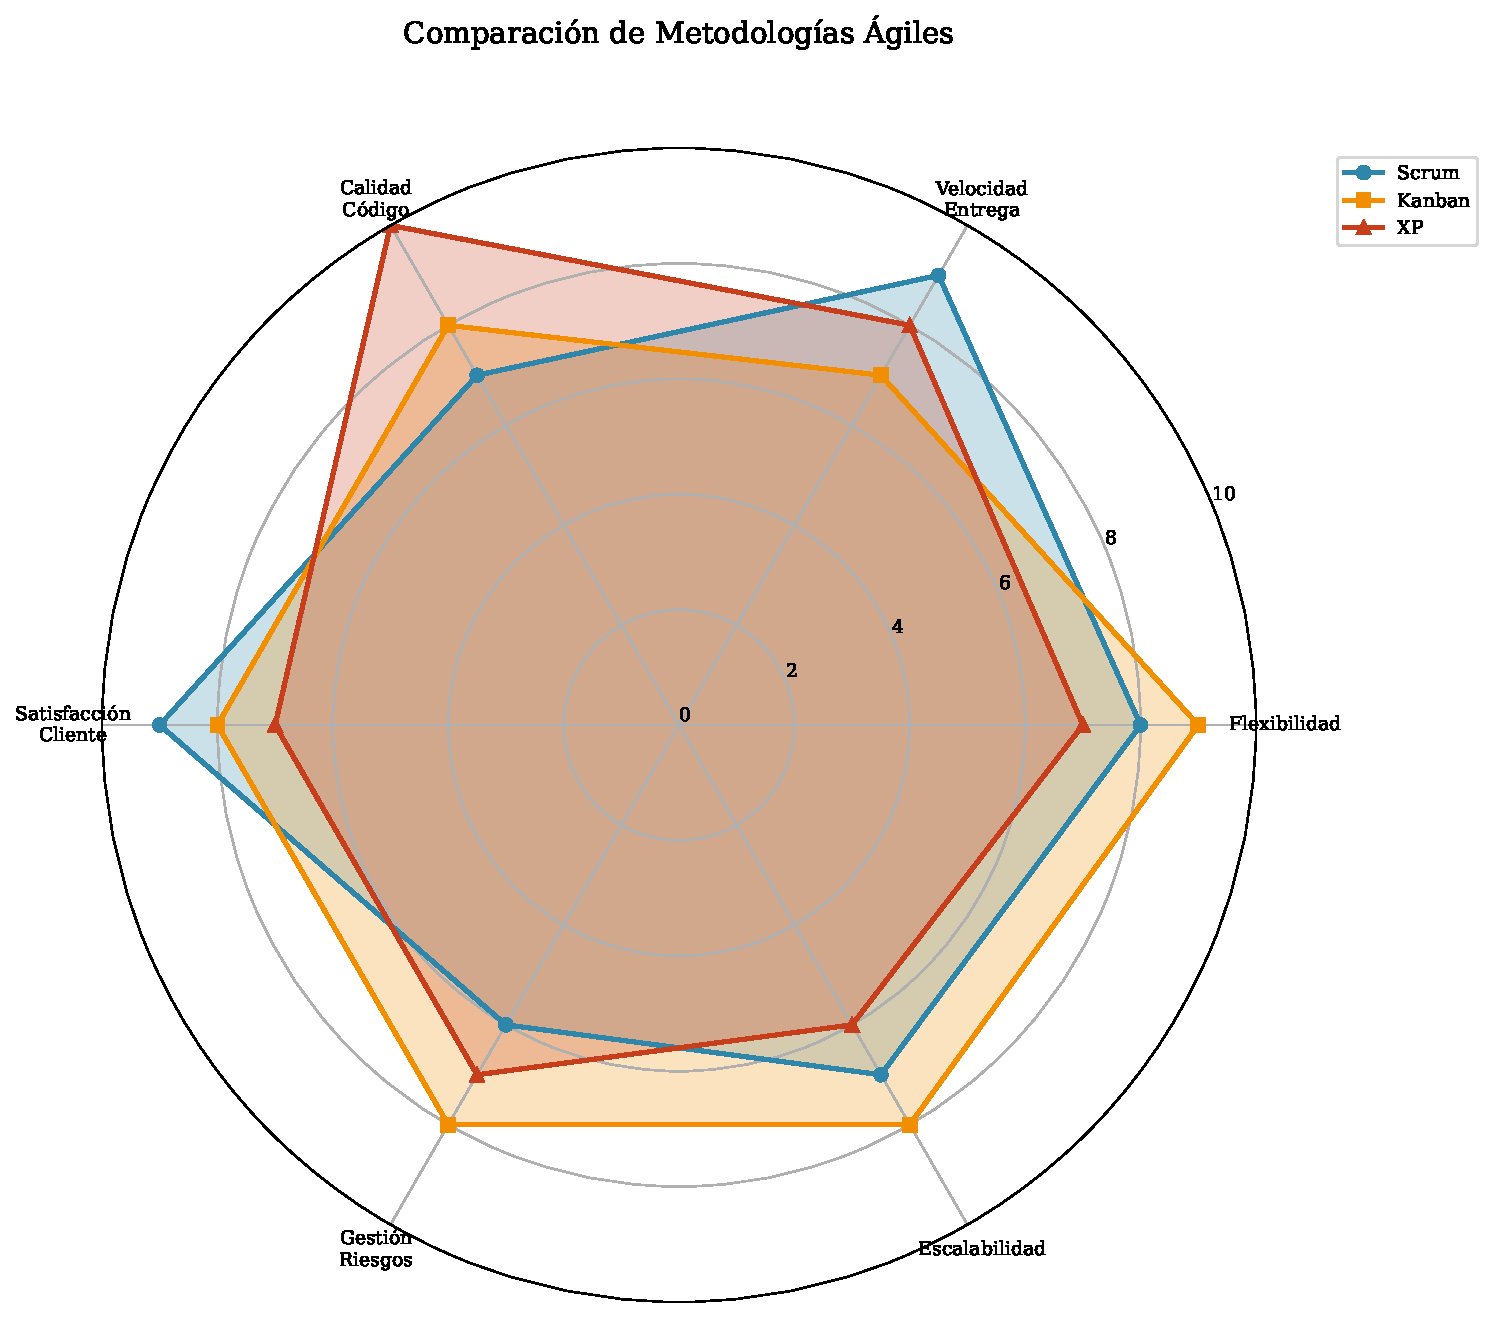
\includegraphics[width=0.45\textwidth]{graphics/comparacion_metodologias.pdf} % Inserta aquí tu gráfico cuando lo tengas
    \caption{Comparación multi-criterio de metodologías ágiles: Scrum, Kanban y XP}
    \label{fig:comparacion_metodologias}
\end{figure}

\subsection{Datos e instrumentos}
Se recolectaron issues, pull requests, pipelines de CI, cobertura de pruebas, defectos y notas de revisión. Se prepararon scripts de extracción/limpieza (carpeta code/) y tablas de síntesis (carpeta tables/). La recolección abarcó un período prolongado del ciclo de desarrollo, combinando métricas cuantitativas con observaciones cualitativas del equipo.

\subsection{Procedimiento y validez}
Se documentaron fases, roles y checkpoints. Para la validez, se consideró:

Interna: consistencia entre cambios y resultados observados.

Externa: aplicabilidad a otras rutas/ciudades con variaciones de conectividad.

De constructo: que las métricas midan lo que declaran medir (p. ej., latencia extremo a extremo).

De conclusión: interpretación prudente de las evidencias.

Mitigaciones de sesgo: anonimización de datos operativos, criterios de aceptación definidos a priori, registro de decisiones y cambios.

Nota sobre el stack y la literatura: el uso de MQTT/WebSockets, APIs documentadas y arquitecturas híbridas se fundamenta en la literatura citada \cite{sismo2016}; \cite{easyrest2022}; \cite{ingenieria2022}, mientras que las comparaciones de herramientas móviles consideran también evidencia reciente en apps multiplataforma \cite{flutter2022new}.